% В этом документе преамбула

\documentclass[a4paper,12pt]{article}

\usepackage{lscape} % горизонтальный режим
\usepackage{pdflscape}

\usepackage{lipsum} % тестовые тексты

%%% Работа с русским языком
\usepackage{cmap}					% поиск в PDF
\usepackage{mathtext} 				% русские буквы в формулах
\usepackage[T2A]{fontenc}			% кодировка
\usepackage[utf8]{inputenc}			% кодировка исходного текста
\usepackage[english,russian]{babel}	% локализация и переносы
\usepackage{indentfirst}			% чтобы первый абзац в разделе отбивался красной строкой
\frenchspacing						% тонкая настройка пробелов
\usepackage{gensymb}				% символы по типу градусов
\usepackage{algorithm}				% для алгоритмов
\usepackage{algorithmic}			% для алгоритмов

%%% Приведение начертания букв и знаков к русской типографской традиции
\renewcommand{\epsilon}{\ensuremath{\varepsilon}}
\renewcommand{\phi}{\ensuremath{\varphi}}			% буквы "эпсилон"
\renewcommand{\kappa}{\ensuremath{\varkappa}}		% буквы "каппа"
\renewcommand{\le}{\ensuremath{\leqslant}}			% знак меньше или равно
\renewcommand{\leq}{\ensuremath{\leqslant}}			% знак меньше или равно
\renewcommand{\ge}{\ensuremath{\geqslant}}			% знак больше или равно
\renewcommand{\geq}{\ensuremath{\geqslant}}			% знак больше или равно
\renewcommand{\emptyset}{\varnothing}				% знак пустого множества

%%% Дополнительная работа с математикой
\usepackage{amsmath,amsfonts,amssymb,amsthm,mathtools,esint} % AMS
\usepackage{wasysym}
\usepackage{icomma} % "Умная" запятая: $0,2$ --- число, $0, 2$ --- перечисление

%% Номера формул
\mathtoolsset{showonlyrefs=true} % Показывать номера только у тех формул, на которые есть \eqref{} в тексте.

%% Свои команды

% операции, не определённые (или имеющие иные обохначения) в мат. пакетах
\DeclareMathOperator{\sgn}{\mathop{sgn}}				% ф-ия sgn
\renewcommand{\tg}{\mathop{\mathrm{tg}}\nolimits}		% обозначение тангенса

%% Перенос знаков в формулах (по Львовскому)
\newcommand*{\hm}[1]{#1\nobreak\discretionary{}
{\hbox{$\mathsurround=0pt #1$}}{}}

%%% Работа с картинками
\usepackage{graphicx}  				% Для вставки рисунков
\graphicspath{{images/}{images2/}}  % папки с картинками
\setlength\fboxsep{3pt} 			% Отступ рамки \fbox{} от рисунка
\setlength\fboxrule{1pt} 			% Толщина линий рамки \fbox{}
\usepackage{wrapfig} 				% Обтекание рисунков текстом

%%% Работа с таблицами
\usepackage{array,tabularx,tabulary,booktabs} 	% Дополнительная работа с таблицами
\usepackage{longtable}  						% Длинные таблицы
\usepackage{multirow}							% Слияние строк в таблице

%%% Теоремы

\newtheoremstyle{break}% name
	{}%         Space above, empty = `usual value'
	{}%         Space below
	{\itshape}% Body font
	{}%         Indent amount (empty = no indent, \parindent = para indent)
	{\bfseries}% Thm head font
	{.}%        Punctuation after thm head
	{\newline}% Space after thm head: \newline = linebreak
	{}%         Thm head spec
\theoremstyle{break}

% \theoremstyle{plain} % Стиль по умолчанию
\newtheorem{theorem}{Теорема}[section]
\newtheorem{lemma}{Лемма}[section]
\newtheorem{definition}[theorem]{Определение}
\newtheorem{property}{Свойство}
 
\newtheorem{corollary}{Следствие}[theorem]

\newtheoremstyle{example}	% style name
	{2ex}					% above space
	{2ex}					% below space
	{}						% body font
	{}						% indent amount
	{\bf}				% head font
	{.}						% post head punctuation
	{\newline}				% post head punctuation
	{\thmname{#1}\thmnumber{ #2}\thmnote{ (#3)}}						% head spec

\theoremstyle{example}
\newtheorem{exmp}{Пример}[section]
 
\theoremstyle{remark} % "Примечание"
\newtheorem*{nonum}{Решение}
\newtheorem*{evidence}{Доказательство}
\newtheorem*{remark}{Примечание}

%%% Программирование
\usepackage{etoolbox} % логические операторы

%%% Страница
\usepackage{extsizes} % Возможность сделать 14-й шрифт
\usepackage{geometry} % Простой способ задавать поля
	\geometry{top=15mm}
	\geometry{bottom=35mm}
	\geometry{left=10mm}
	\geometry{right=10mm}

%\usepackage{fancyhdr} % Колонтитулы
% 	\pagestyle{fancy}
 	%\renewcommand{\headrulewidth}{0pt}  % Толщина линейки, отчеркивающей верхний колонтитул
% 	\lfoot{Нижний левый}
% 	\rfoot{Нижний правый}
% 	\rhead{Верхний правый}
% 	\chead{Верхний в центре}
% 	\lhead{Верхний левый}
%	\cfoot{Нижний в центре} % По умолчанию здесь номер страницы

\usepackage{setspace} % Интерлиньяж (межстрочные интервалы)
%\onehalfspacing % Интерлиньяж 1.5
%\doublespacing % Интерлиньяж 2
%\singlespacing % Интерлиньяж 1

\usepackage{lastpage} % Узнать, сколько всего страниц в документе.

\usepackage{soulutf8} % Модификаторы начертания

\usepackage{hyperref}
\usepackage[usenames,dvipsnames,svgnames,table,rgb]{xcolor}
\hypersetup{				% Гиперссылки
    unicode=true,           % русские буквы в раздела PDF
    pdftitle={Заголовок},   % Заголовок
    pdfauthor={Автор},      % Автор
    pdfsubject={Тема},      % Тема
    pdfcreator={Создатель}, % Создатель
    pdfproducer={Производитель}, % Производитель
    pdfkeywords={keyword1} {key2} {key3}, % Ключевые слова
    colorlinks=true,       	% false: ссылки в рамках; true: цветные ссылки
    linkcolor=MidnightBlue, % внутренние ссылки
    citecolor=black,        % на библиографию
    filecolor=magenta,      % на файлы
    urlcolor=blue           % на URL
}

\usepackage{csquotes} % Еще инструменты для ссылок

%\usepackage[style=authoryear,maxcitenames=2,backend=biber,sorting=nty]{biblatex}

\usepackage{multicol} % Несколько колонок

%%% Работа с графикой
\usepackage{tikz}
\usetikzlibrary{calc}
\usepackage{tkz-euclide}
\usetikzlibrary{arrows}
\usepackage{pgfplots}
\usepackage{pgfplotstable}

%%% Настройка подписей к плавающим объектам
% \usepackage{floatrow}	% размещение
\usepackage{caption}	% начертание
\captionsetup[figure]{labelfont=bf,textfont=it,font=footnotesize}	% нумерация и надпись курсивом
% для подфигур: заголовок подписи полужирный, текст заголовка обычный
% выравнивание является неровным (т.е. выровненным по левому краю)
% singlelinecheck = off означает, что настройка выравнивания используется, даже если заголовок имеет длину только одну строку.
% если singlelinecheck = on, то заголовок всегда центрируется, когда заголовок состоит только из одной строки.
\captionsetup[subfigure]{labelfont=bf,textfont=normalfont,singlelinecheck=off,justification=raggedright}

%%% Stuff для листинга
\usepackage{listings}
\usepackage{xcolor}

\colorlet{mygray}{black!30}
\colorlet{mygreen}{green!60!blue}
\colorlet{mymauve}{red!60!blue}

\lstset{
	backgroundcolor=\color{gray!10},  
	basicstyle=\ttfamily,
	columns=fullflexible,
	breakatwhitespace=false,      
	breaklines=true,                
	captionpos=b,                    
	commentstyle=\color{mygreen}, 
	extendedchars=true,              
	frame=single,                   
	keepspaces=true,             
	keywordstyle=\color{blue},      
	language=c++,                 
	numbers=none,                
	numbersep=5pt,                   
	numberstyle=\tiny\color{blue}, 
	rulecolor=\color{mygray},        
	showspaces=false,               
	showtabs=false,                 
	stepnumber=5,                  
	stringstyle=\color{mymauve},    
	tabsize=3,                      
	title=\lstname                
}

% для извращённых начертаний
\usepackage{mathrsfs}

\usepackage{makecell}
\setcellgapes{3pt}

% Зачёркивание символов
\usepackage{cancel}

% перечисления с буквами
\usepackage{enumitem}

\title{Теория вероятностей и мат. статистика}
\date{16.05.2020}
\author{Почаев Никита Алексеевич, гр. 8381 \\ \href{mailto:pochaev.nik@gmail.com}{pochaev.nik@gmail.com} \\ Преподаватель: Малов Сергей Васильевич}

\begin{document}
	
\renewcommand{\figurename}{Рисунок}

\maketitle

\section*{Независимость случайных величин и условные распределения}

\subsection*{Задача 6 (СГТВ 4.7)}

\noindent\textbf{Условие:}

Случайный вектор $(\xi, \eta)$ имеет двухмерное дискретное распределение, заданное таблицами (варианты а) и б)):
\begin{figure}[h]
	\center{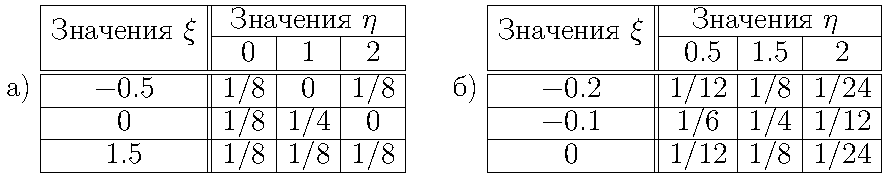
\includegraphics[scale=1]{./media/task_4_7.pdf}}
\end{figure}

Проверить, являются ли компоненты вектора $(\xi, \eta)$ независимыми; вычислить условные распределения $\xi$ при условии $\eta$ и $\eta$ при условии $\xi$, а также коэффициент корреляции $r(\xi, \eta)$ и условное математическое ожидание $\xi$ при различных значениях $\eta$.

\noindent\textbf{Решение:}

\begin{enumerate}
	\item[а)]
	Представим распределение компонент в виде таблиц:
	\begin{table}[H]
		\centering
		\begin{tabular}{|c|c|c|c|}
			\hline
			$\xi$ & -0.5 & 0   & 1.5 \\ \hline
			$P$   & 2/8  & 3/8 & 3/8 \\ \hline
		\end{tabular}
	\end{table}
	\begin{table}[H]
		\centering
		\begin{tabular}{|c|c|c|c|}
			\hline
			$\eta$ & 0   & 1   & 2   \\ \hline
			$P$    & 3/8 & 3/8 & 2/8 \\ \hline
		\end{tabular}
	\end{table}
	
	Покажем, что случайные величины являются зависимыми, например:
	\[ P(\xi = -0.5, \eta = 0) = \frac{1}{8}; ~~~~~~ P(\xi = -0.5) \cdot P(\eta = 0) = \frac{2}{8} \cdot \frac{3}{8} = \frac{3}{32} \]
	\[ \frac{1}{8} = P(\xi = -0.5, \eta = 0) \ne P(\xi = -0.5) \cdot P(\eta = 0) = \frac{3}{32} \]
	
	Компоненты случайного вектора могут быть независимыми только если любой носитель его распределения с точностью до событий вероятности 0 представляется как прямое произведение носителей распределений компонент, что в данном случае не выполняется.
	
	Вычислим мат. ожидание:
	\[
	E\xi = -0.5 \cdot \frac{2}{8} + 0 \cdot \frac{3}{8} + 1.5 \cdot \frac{3}{8} = \frac{7}{16};
	~~~~~~
	E\eta = 0 \cdot \frac{3}{8} + 1 \cdot \frac{3}{8} + 2 \cdot \frac{2}{8} = \frac{7}{8}
	\]
	\[ E\xi\eta = -0.5 \cdot 2 \cdot \frac{1}{8} + 1.5 \cdot 1 \cdot \frac{1}{8} + 1.5 \cdot 2 \cdot \frac{1}{8} = \frac{7}{16} \]
	
	Найдём меру линейной зависимости двух случайных величин - ковариацию:
	\[ \cov (\xi, \eta) = E\xi\eta - E\xi \cdot E\eta = \frac{7}{16} - \frac{7}{16} \cdot \frac{7}{8} = \frac{7}{128} \]
	
	Вычислим дисперсию:
	\[
	E\xi^2 = \frac{1}{4} \cdot \frac{2}{8} + \frac{9}{4} \cdot \frac{3}{8} = \frac{29}{32}
	~~~~~~
	E\eta^2 = \frac{3}{8} + 4 \cdot \frac{2}{8} = \frac{11}{8}
	\]
	\[
	D\xi = E\xi^2 - (E\xi)^2 = \frac{29}{32} - \left( \frac{7}{16} \right)^2 = \frac{183}{256}
	~~~~~~
	D\eta = E\eta^2 - (E\eta)^2 = \frac{11}{8} - \left( \frac{7}{8} \right)^2 =\frac{39}{64}
	\]
	
	Найдём коэффициент корреляции:
	\[ r(\xi, \eta) = \frac{\cov (\xi, \eta)}{\sqrt{D\xi \cdot D\eta}} = \frac{\frac{7}{128}}{\sqrt{\frac{183}{256} \cdot \frac{39}{64}}} = \frac{7 \sqrt{793}}{2379} \approx 0.0828591 \]
	Т.к. коэффициент корреляции близится к 0, то между величинами наблюдается слабая зависимость. Иными словами, поведение величины $\xi$ не будет совсем (или почти совсем) влиять на поведение $\eta$ (и наоборот).
	
	Матрица ковариации:
	\[
	\var \begin{pmatrix} \xi \\ \eta \end{pmatrix} =
	\begin{pmatrix}
	183/256 & 7/128 \\
	7/128 & 39/64
	\end{pmatrix}
	\]
	
	Далее распишем условные распределения $\xi$ при условии $\eta$ и наоборот соотвественно.
	
	\[
	q_{\xi | \eta = y} (x) = \frac{P(\xi = x, \eta = y)}{P(\eta = y)} (x=\{ -0.5, 0, 1,5 \}, y = \{ 0, 1, 2 \})
	\]
	\[
	q_{\eta | \xi = y} (x) = \frac{P(\xi = y, \eta = x)}{P(\xi = y)} (x = \{ 0, 1, 2 \}, y = \{ -0.5, 0, 1.5 \})
	\]
	
	\begin{table}[H]
		\centering\makegapedcells
		\begin{tabular}{|c|c|c|c|}
			\hline
			\diagbox{Знач. $\xi$}{Знач. $\eta$} & 0                             & 1                             & 2                             \\ \hline
			-0.5                                & $\frac{1/8}{3/8}=\frac{1}{3}$ & 0                             & $\frac{1/8}{2/8}=\frac{1}{2}$ \\ \hline
			0                                   & $\frac{1/8}{3/8}=\frac{1}{3}$ & $\frac{1/4}{3/8}=\frac{2}{3}$ & 0                             \\ \hline
			1.5                                 & $\frac{1/8}{3/8}=\frac{1}{3}$ & $\frac{1/8}{3/8}=\frac{1}{3}$ & $\frac{1/8}{2/8}=\frac{1}{2}$ \\ \hline
		\end{tabular}
	\end{table}
	\begin{table}[H]
		\centering\makegapedcells
		\begin{tabular}{|c|c|c|c|}
			\hline
			\diagbox{Знач. $\eta$}{Знач. $\xi$} & -0.5                          & 0                             & 1.5                           \\ \hline
			0                                   & $\frac{1/8}{2/8}=\frac{1}{2}$ & $\frac{1/8}{3/8}=\frac{1}{3}$ & $\frac{1/8}{3/8}=\frac{1}{3}$ \\ \hline
			1                                   & 0                             & $\frac{1/4}{3/8}=\frac{2}{3}$ & $\frac{1/8}{3/8}=\frac{1}{3}$ \\ \hline
			2                                   & $\frac{1/8}{2/8}=\frac{1}{2}$ & 0                             & $\frac{1/8}{3/8}=\frac{1}{3}$ \\ \hline
		\end{tabular}
	\end{table}
	Нетрудно заметить, что в обоих случаях сумма значений по столбцам даёт единицу.
	
	Условное математическое ожидание $\xi$ при различных значениях $\eta$:
	\[
	E(\xi | \eta = 0) = -0.5 \cdot \frac{1}{3} + 1.5 \cdot \frac{1}{3} = \frac{1}{3};
	~~~~~~
	D(\xi | \eta = 0) = 0.25 \cdot \frac{1}{3} + 2.25 \cdot \frac{1}{3} - \left( \frac{1}{3} \right)^2 = \frac{13}{18}
	\]
	\[
	E(\xi | \eta = 1) = \frac{1}{3} \cdot 1.5 = \frac{1}{2};
	~~~~~~
	D(\xi | \eta = 1) = 2.25 \cdot \frac{1}{3} - \left( \frac{1}{2} \right)^2 = \frac{1}{2}
	\]
	\[
	E(\xi | \eta = 2) = -0.5 \cdot \frac{1}{2} + 1.5 \cdot \frac{1}{2} = \frac{1}{2};
	~~~~~~
	D(\xi | \eta = 2) = 0.25 \cdot \frac{1}{2} + 2.25 \cdot \frac{1}{2} - \left( \frac{1}{2} \right)^2 = 1
	\]
	
	Распределение $E(\xi | \eta)$:
	\begin{table}[H]
		\centering\makegapedcells
		\begin{tabular}{|c|c|c|}
			\hline
			$E(\xi | \eta)$ & $\frac{1}{3}$ & $\frac{1}{2}$ \\ \hline
			$P$             & $\frac{3}{8}$ & $\frac{5}{8}$ \\ \hline
		\end{tabular}
	\end{table}
	
	Распределение $D(\xi | \eta)$:
	\begin{table}[H]
		\centering\makegapedcells
		\begin{tabular}{|c|c|c|c|}
			\hline
			$D(\xi | \eta)$ & $\frac{1}{2}$ & $\frac{13}{18}$ & 1             \\ \hline
			$P$             & $\frac{3}{8}$ & $\frac{3}{8}$   & $\frac{2}{8}$ \\ \hline
		\end{tabular}
	\end{table}

	\item[б)] Распределение компонент представлено ниже:
	\begin{table}[H]
		\centering
		\begin{tabular}{|c|c|c|c|}
			\hline
			$\xi$ & -0.2 & -0.1 & 0   \\ \hline
			$P$   & 1/4  & 1/2  & 1/4 \\ \hline
		\end{tabular}
	\end{table}
	\begin{table}[H]
		\centering
		\begin{tabular}{|c|c|c|c|}
			\hline
			$\eta$ & 0.5 & 1.5 & 2   \\ \hline
			$P$    & 1/3 & 1/2 & 1/6 \\ \hline
		\end{tabular}
	\end{table}

	Проверим независимость:
	\begin{table}[H]
		\centering
		\begin{tabular}{|c|c|c|c|}
			\hline
			\diagbox{Знач. $\xi$}{Знач. $\eta$} & 0.5                                            & 1.5                                           & 2                                              \\ \hline
			-0.2                                & $\frac{1}{4} \cdot \frac{1}{3} = \frac{1}{12}$ & $\frac{1}{4} \cdot \frac{1}{2} = \frac{1}{8}$ & $\frac{1}{4} \cdot \frac{1}{6} = \frac{1}{24}$ \\ \hline
			-0.1                                & $\frac{1}{2} \cdot \frac{1}{3} = \frac{1}{6}$  & $\frac{1}{2} \cdot \frac{1}{2} = \frac{1}{4}$ & $\frac{1}{2} \cdot \frac{1}{6} = \frac{1}{12}$ \\ \hline
			0                                   & $\frac{1}{4} \cdot \frac{1}{3} = \frac{1}{12}$ & $\frac{1}{4} \cdot \frac{1}{2} = \frac{1}{8}$ & $\frac{1}{4} \cdot \frac{1}{6} = \frac{1}{24}$ \\ \hline
		\end{tabular}
	\end{table}
	Как видно из таблиц, $P(\xi, \eta) = P(\xi) \cdot P(\eta) \Rightarrow$ величины независимы.
	
	Найдём мат. ожидание:
	\[
	E\xi = -0.2 \cdot \frac{1}{4} - 0.1 \cdot \frac{1}{2} = - \frac{1}{10};
	~~~~~~
	E\xi^2 = 0.04 \cdot \frac{1}{4} + 0.01 \cdot \frac{1}{2} = \frac{3}{200}
	\]
	\[
	E\eta = 0.5 \cdot \frac{1}{3} + 1.5 \cdot \frac{1}{2} + 2 \cdot \frac{1}{6} = \frac{5}{4};
	~~~~~~
	E\eta^2 = 0.25 \cdot \frac{1}{3} + 2.25 \cdot \frac{1}{2} + 4 \cdot \frac{1}{6} = \frac{15}{8}
	\]
	\[
	E\xi\eta = -0.2 \cdot \left( 0.5 \cdot \frac{1}{12} + 1.5 \cdot \frac{1}{8} + 2 \cdot \frac{1}{24} \right) - 0.1 \cdot \left( 0.5 \cdot \frac{1}{6} + 1.5 \cdot \frac{1}{4} + 2 \cdot \frac{1}{12} \right) = -\frac{1}{6}
	\]
	Дисперсия:
	\[
	D\xi = E\xi^2 - (E\xi^2) = \frac{3}{200} - \left( -\frac{1}{10} \right)^2  = 0.005;
	~~~
	D\eta = E\eta^2 - (E\eta^2) = \frac{15}{8} - \left( \frac{5}{4} \right)^2 = 0.3125
	\]
	Ковариация:
	\[ \cov (\xi, \eta) = E\xi\eta - E\xi \cdot E\eta = - \frac{1}{6} + \frac{1}{10} \cdot \frac{5}{4} = -\frac{1}{24} \]
	Коэффициент корреляции:
	\[ r (\xi, \eta) = \frac{\cov (\xi, \eta)}{\sqrt{D\xi \cdot D\eta}} = \frac{-\frac{1}{24}}{\sqrt{0.005 \cdot 0.3125}} = - \frac{- \sqrt{10}}{3} \approx - 1.05409 \]
	Матрица ковариации:
	\[
	\var \begin{pmatrix} \xi \\ \eta \end{pmatrix} =
	\begin{pmatrix}
		0.005 & - \frac{1}{24} \\
		- \frac{1}{24} & 0.3125
	\end{pmatrix}
	\]
	
	Далее распишем условные распределения $\xi$ при условии $\eta$ и наоборот соотвественно.
	\begin{table}[H]
		\centering
		\begin{tabular}{|c|c|c|c|}
			\hline
			\diagbox{Знач. $\xi$}{Знач. $\eta$} & 0.5                            & 1.5                           & 2                              \\ \hline
			-0.2                                & $\frac{1/12}{1/3}=\frac{1}{4}$ & $\frac{1/8}{1/2}=\frac{1}{4}$ & $\frac{1/24}{1/6}=\frac{1}{4}$ \\ \hline
			-0.1                                & $\frac{1/6}{1/3}=\frac{1}{2}$  & $\frac{1/4}{1/2}=\frac{1}{2}$ & $\frac{1/12}{1/6}=\frac{1}{2}$ \\ \hline
			0                                   & $\frac{1/12}{1/3}=\frac{1}{4}$ & $\frac{1/8}{1/2}=\frac{1}{4}$ & $\frac{1/24}{1/6}=\frac{1}{4}$ \\ \hline
		\end{tabular}
	\end{table}
	\begin{table}[H]
		\centering
		\begin{tabular}{|c|c|c|c|}
			\hline
			\diagbox{Знач. $\eta$}{Знач. $\xi$} & -0.2                           & -0.1                           & 0                              \\ \hline
			0.5                                 & $\frac{1/12}{1/4}=\frac{1}{3}$   & $\frac{1/6}{1/2}=\frac{1}{3}$  & $\frac{1/12}{1/4}=\frac{1}{3}$ \\ \hline
			1.5                                 & $\frac{1/8}{1/4}=\frac{1}{2}$    & $\frac{1/4}{1/2}=\frac{1}{2}$  & $\frac{1/8}{1/4}=\frac{1}{2}$  \\ \hline
			2                                   & $\frac{1/24}{1/4}=\frac{1}{6}$ & $\frac{1/12}{1/2}=\frac{1}{6}$ & $\frac{1/24}{1/4}=\frac{1}{6}$ \\ \hline
		\end{tabular}
	\end{table}
	Как нетрудно заметить сумма элементов по столбцам даёт единицу, а одинаковые значения по строкам подтверждают независимость компонент.
	
	Условное математическое ожидание $\xi$ при различных значениях $\eta$:
	\[
	E(\xi | \eta = 0.5) = -0.2 \cdot \frac{1}{4} - 0.1 \cdot \frac{1}{2} = -0.1;
	~~~
	E(\xi | \eta = 1.5) = -0.2 \cdot \frac{1}{4} - 0.1 \cdot \frac{1}{2} = -0.1
	\]
	\[
	E(\xi | \eta = 2) = -0.2 \cdot \frac{1}{4} - 0.1 \cdot \frac{1}{2} = -0.1
	\]
	
	\[
	D(\xi | \eta = 0.5) = D(\xi | \eta = 1.5) = D(\xi | \eta = 2) = 0.04 \cdot \frac{1}{4} + 0.01 \cdot \frac{1}{2} - 0.01 = 0.005;
	\]
\end{enumerate}

\subsection*{Задача 7 (СГТВ 4.8)}

Проверить, являются ли независимыми компоненты вектора $(\xi, \eta)$; вычислить условные распределения $\xi$ при условии $\eta$ и $\eta$ при условии $\xi$ и коэффициент корреляции $r(\xi, \eta)$, если их совместная плотность распределения имеет вид:
\begin{enumerate}
	\item[а)]
	\[
	p_{\xi, \eta} (x, y) =
	\begin{cases}
		|x-y|/3, x,y \in [0,1] \\
		0 - \text{ в остальных случаях}
	\end{cases}
	\]
	\item[б)]
	\[
	p_{\xi, \eta} (x, y) =
	\begin{cases}
		c \exp (- (x + y)), 0 \le x \le y \\
		0 - \text{ в остальных случаях}
	\end{cases}
	\]
	\item[в)]
	\[
	p_{\xi, \eta} (x, y) =
	\frac{1}{2 \pi \sigma_1 \sigma_2 \sqrt{1 - \rho^2}} \exp \left[ - \frac{1}{2 (2 - \rho^2)} \left( \frac{x^2}{\rho_1^2} - 2 \rho \frac{xy}{\sigma_1 \sigma_2} + \frac{y^2}{\sigma_2^2} \right) \right]
	\]
	\[ x, y \in \mathbb{R}, \text{ где } \sigma_1, \sigma_2 > 0, \rho \in (-1, 1) - \text{ некоторые параметры.} \]
\end{enumerate}

\end{document} 